%\documentclass{article}
\documentclass[            %% KOMA-Skript Dokumentklassen verwenden
draft = false,             		% Entwurfsmodus
paper = A4,                		% Papierart
% paper = landscape,       		% Seite im Querformat setzen
pagesize = pdftex,         		% Pagesize an pdfTeX anpassen
% pagesitze = xetex,       		% Pagesize an XeTeX anpassen
fontsize = 10pt,           		% Schriftgröße (12pt, 11pt (Standard))
%BCOR = 10mm,                	% Bindekorrektur
DIV=15,                    		% Satzspiegelfaktor, je größer, desto mehr Text auf Seite
twoside = false,           		% Doppelseiten (Ein|Aus|Semi)
twocolumn = false,         		% zweispaltiger Satz
parskip = full,           		% Absatzformatierung s. scrguide 3.1
%abstract = true,         		% Überschrift über Abstract an (nicht bei scrbook aktiv)
chapterprefix = false,      		% Layout der Kapitelüberschriften
appendixprefix = true,     		% Layout der Anhangüberschriften
headinclude = false,       		% Kopfzeile zu Text betrachten (für Satzspiegelberechnung)
footinclude = false,       		% Fußzeile zu Text betrachten (für Satzspiegelberechnung)
mpinclude = false,         		% Rand zum Text betrachten (für Satzspiegelberechnung)
% headlines = 1.25,        		% Anzahl der Kopfzeilen
% headheight = 2cm,        		% Höhe der Kopfzeile
% headsepline = true,      		% Trennline zum Seitenkopf
% footsepline = true,      		% Trennline zum Seitenfuß
numbers = auto,            		% KOMA-Skript setzt Endpunktierung im Inahltsverzeichnis.
cleardoublepage = plain,   		% Einstellung des Seitenstils für eingefügte Vakatseiten
% leqno,                   		% Nummerierung von Gleichungen links
% fleqn,                   		% Ausgabe von Gleichungen linksbündig
footnotes = multiple,      		% Mehrer aufeinander folgende Fußnoten durch Komma trennen
titlepage = true,          		% Titelei auf eigener Seite \maketitle[Seitenanzahl]
%headings = openright,     		% Kapitel auf rechter Seite beginnen, ggf. Vakatseiten
headings = normal,         		% Normalgroße Überschriften
open = right,              		% Seiten rechts beginnen
%toc = listof,
%toc = listof,              		% Abb.- und Tab.verzeichnis im Inhaltsverzeichnis
%toc = noindex,             		% Index im Inhaltsverzeichnis (index|noindex)
%toc = sectionentrywithoutdots,
%toc = chapterentrywithoutdots,
bibliography = openstyle,  		% Offener Darstellungsstil der Bibliographie
listof = chaptergapline,   		% Abb.- und Tab.verzeichnis werden nach Kapitel geordnet
overfullrule = true,
]{scrbook}

\usepackage{mathtools}
\usepackage{amssymb}

\usepackage[ngerman]{babel}
%\usepackage[ansinew]{inputenc}

\usepackage[pdftex]{graphicx}			% Zum Laden von Grafiken
\graphicspath{{Bilder/}}				% Standardpfad für Bilder/Grafiken

% for captions outside of floats in minipage
% https://tex.stackexchange.com/questions/57433/cannot-use-caption-under-minipage
\usepackage{caption}

% Bibliographiestil %%%%%%%%%%%%%%%%%%%%%%%%%%%%%%%%%%%%%%%%%%%%%%%%%%%%%%%%%%%%%%%%
\usepackage[				% Erweiterung der Basisfunktionalität
	numbers,				% Nummern
   %authoryear,
	square,					% Eckige Klammern
%    sort&compress,			% Multiple Zitate sortieren und zusammenfassen
%    longnamesfirst			% Erstes Zitat mit vollen Namen
   ]
   {natbib}

%{Bibliographie/ka-style}
   \setcitestyle{
%     authoryear,% Author-Year-Style
%      square,   % Eckige Klammern
%     semicolon, % semicolon als Trennzeichen
      aysep{},% Kein explizites Trennzeichen zwischen Author und Year
      yysep{;}% Komma als Trennzeichen zwischen mehreren Jahren
      }

% break long URLs in the bibliography
\usepackage{url}
\def\UrlBreaks{\do\/\do-}

% For TODO markers
\usepackage{todonotes}

% for C code listings
% https://tex.stackexchange.com/questions/348651/c-code-to-add-in-the-document
\usepackage{xcolor}
\usepackage{listings}

% https://tex.stackexchange.com/questions/370334/use-color-in-verbatim-environment
\usepackage{fancyvrb}
\usepackage{xcolor}

\definecolor{mGreen}{rgb}{0,0.6,0}
\definecolor{mGray}{rgb}{0.5,0.5,0.5}
\definecolor{mPurple}{rgb}{0.58,0,0.82}
\definecolor{arduino_green}{rgb}{0, 0.6, 0.756}
\definecolor{arduino_string}{rgb}{0, 0.36, 0.37}
\definecolor{backgroundColour}{rgb}{1.0, 1.0, 1.0}

\lstdefinestyle{CStyle}{
    backgroundcolor=\color{backgroundColour},   
    commentstyle=\color{mGreen},
    keywordstyle=\color{arduino_green},
    numberstyle=\tiny\color{mGray},
    stringstyle=\color{arduino_string},
    basicstyle=\footnotesize,
    breakatwhitespace=false,         
    breaklines=true,                 
    captionpos=b,                    
    keepspaces=true,                 
    numbers=left,                    
    numbersep=5pt,                  
    showspaces=false,                
    showstringspaces=false,
    showtabs=false,                  
    tabsize=2,
    language=C
}


\makeatletter
\newcommand{\faculty}[1]{\gdef\@faculty{#1}}
\newcommand{\@faculty}{\@latex@warning@no@line{No \noexpand\faculty given}}
\newcommand{\thesisType}[1]{\gdef\@thesisType{#1}}
\newcommand{\@thesisType}{\@latex@warning@no@line{No \noexpand\thesisType given}}
\newcommand{\erstpruefer}[1]{\gdef\@erstpruefer{#1}}
\newcommand{\@erstpruefer}{\@latex@warning@no@line{No \noexpand\erstpruefer given}}
\newcommand{\zweitpruefer}[1]{\gdef\@zweitpruefer{#1}}
\newcommand{\@zweitpruefer}{\@latex@warning@no@line{No \noexpand\zweitpruefer given}}
\newcommand{\matrikelnummer}[1]{\gdef\@matrikelnummer{#1}}
\newcommand{\@matrikelnummer}{\@latex@warning@no@line{No \noexpand\matrikelnummer given}}


\newcommand{\addtotoc}[1]{
\addcontentsline{toc}{chapter}{
   \texorpdfstring{
      \MakeUppercase{#1}
   }{#1}
   }
}







\begin{document}



\overfullrule=0mm



\author{Markus Goeritzer, Patrick Freidhof, Wolfgang Bischoff}
\title{Regelungstechnik Praktikum}
\subject{Bode Diagram}
\thesisType{Praktikumsbericht}
\faculty{Fakultät Ingenieurswissenschaften}
\erstpruefer{???}
%\zweitpruefer{???}
\matrikelnummer{???, ???, 2228538}

\begin{center}
   \makeatletter
   \underline{\@title}
   \makeatother
\end{center}

\begin{flushleft}

   % author
   \vspace{4em}
   Autor:\\
   \makeatletter
   \@author\\
   \@matrikelnummer\\
   \makeatother

   % Bild
   \vspace{1em}
   \begin{center}
      \begin{minipage}[b]{0.8\textwidth}
         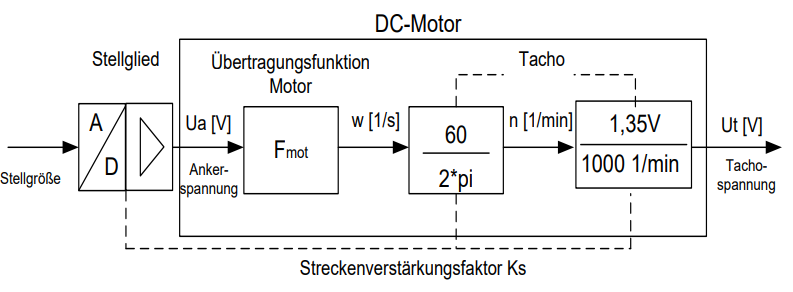
\includegraphics[scale=0.8]{Bilder/TitlePicture.png}
      \end{minipage}
   \end{center}

   % pruefer
   \vspace{9em}
   \underline{Erstprüfer:}\\
   \makeatletter
   \@erstpruefer\\
   \makeatother
   \vspace{1em}
%     \underline{Zweitprüfer/Externer Gutachter:} \\
%     \makeatletter
%     \@zweitpruefer\\
   \makeatother
   \vspace{9em}
   \begin{minipage}[b]{0.4\textwidth}
      
\includegraphics[scale=0.15]{Bilder/thab_logo.png}
   \end{minipage}
   \par
   \large{\MakeUppercase{\textbf{Technische Hochschule Aschaffenburg}}} \par
   \makeatletter
   \large{\MakeUppercase{\textbf{\@faculty}}} \par
   \makeatother
   \large{\MakeUppercase{\textbf{Würzburger Straße 45}}} \par
   \large{\MakeUppercase{\textbf{D-63743 Aschaffenburg}}} \par
   \vfill
\end{flushleft}

% remove page numbering! Has to be placed after all other commands!
\thispagestyle{empty}




\newpage

%\listoftodos

% remove page numbering! Has to be placed after all other commands!
\thispagestyle{empty}





\newpage



\tableofcontents

\vspace{250px}

\textbf{Erklärung zum Praktikumsbericht}

Hiermit versichere ich, dass ich die vorliegende Arbeit selbständig verfasst
und keine anderen Hilfsmittel als die angegebenen verwendet habe.
Die Stellen, die anderen Werken
(gilt ebenso für Werke aus elektronischen Datenbanken oder aus dem Internet)
wörtlich oder sinngemäß entnommen sind, habe ich unter Angabe der Quelle
und Einhaltung der Regeln wissenschaftlichen Zitierens kenntlich gemacht.
Diese Versicherung umfasst auch in der Arbeit verwendete bildliche Darstellungen,
Tabellen, Kartenskizzen und gelieferte Zeichnungen.

Mir ist bewusst, dass Täuschungen nach der für mich gültigen Studien- und
Prüfungsordnung / nach § 6 RaPO / § 48 BayVwVfG geahndet werden.

Die Zustimmung zur elektronischen Plagiatsprüfung wird erteilt.
\vspace{1.5cm}

\begin{tabular}{@{}p{3.5cm}p{7cm}@{}}
 \hrulefill & \hrulefill \\
 Ort, Datum & Unterschrift des Verfassers / der Verfasserin \\
\end{tabular}

% remove page numbering! Has to be placed after all other commands!
\thispagestyle{empty}




\newpage

\pagenumbering{arabic}
\setcounter{page}{1} % Set the page counter to 1

%\newpage

%\chapter{Einleitung} \label{chpt:Einleitung_Main}
{\let\clearpage\relax \chapter{Einleitung}} \label{chpt:Einleitung_Main}

%\todo{Rechtschreibprüfung mit Word}

Dieser Bericht beschreibt die Durchführung des interdisziplinären Praktikums im Fach Regelungstechnik an der TH Aschaffenburg 
im Rahmen des Studiums der Elektro- und Informationstechnik (Berufsbegleitend) EIBB.

Aus der gegebenen Themenauswahl wurde das Thema ``Reglereinstellung im Bodediagramm'' eines Elektronischen Antriebs gewählt. 
Hierbei wird das Verhalten von Übertragungsgliedern (Regler, Steuerung in Kombination mit der Strecke) im Frequenzbereich untersucht.
Dazu wird das System zunächst methodisch untersucht und dann das Eingangssignal mit dem resultierenden Ausgangssignal auch messtechnisch verglichen.
Aus den gewonnenen Erkenntnissen werden Parameter für eine Regelung der Strecke abgeleitet, die ein gewünschtes Verhalten haben soll.


\newpage
{\let\clearpage\relax \chapter{Theoretische Grundlagen}} \label{chpt:Theory}

Brauchen wir dieses Kapitel?







%\newpage
{\let\clearpage\relax \chapter{Aufgaben zur Vorbereitung des Praktikum}} \label{chpt:Experiments}

%%
%% Aufgabe 1 - Übertragungsfunktion
%%

\paragraph{Aufgabe 1 - Übertragungsfunktion}~\\

Gesucht ist die Übertragungsfunktion der Strecke.

Gegeben ist die Differentialgleichung der Strecke und vorläufige Parameter, die während der Vorbereitung des Praktikum zu verwenden sind und
später während der Versuchsdurchführung zu bestimmen sind.

Es werden noch zusätzliche Annahmen getroffen.

Annahme 1: Frequenzgangfunktion und Übertragungsfunktion sind Synonyme.
Grund: \cite{versuchssanleitung} Seite 10. Hinweise: ``tf (...) definiert eine Übertragungs- bzw. Frequenzgangfunktion''

Annahme 2: Wir gehen davon aus, dass bei der Überführung der Differentialgleichung zur Laplace-Übertragungsfunktion, die Terme mit den Anfangswerten entfallen.
Grund: \cite{Skript_Regelungstechnik} Seite 41. ``Da man in der Regelungstechnik meist davon ausgeht, dass sich die betrachteten Systeme für $t < 0$ 
in Nullage befinden [...] verschwinden die Terme mit den Anfangswerten''.

Zur Lösung dieser Aufgabe verwenden wir die gegebene Differentialgleichung.

\begin{equation}
T_1 * T_2 * \ddot x_a(t) + (T_1 + T_2) * \dot x_a(t) + x_a(t) = K_s * x_e(t)
\end{equation}

mit den gegebenen Werten 

$T_1=600 ms; T_2 = 10 ms; K_s = 0,5$

Es handelt sich hier um ein allgemeines $PT_{2}$ Glied siehe \cite{Skript_Regelungstechnik} Seite 68.

Die Übertragungsfunktion wird durch Gleichung 6.6 in \cite{Skript_Regelungstechnik} Seite 69 angegeben als 

\begin{equation}
G(s) = \frac{K}{1 + (T_1 + T_2)s + T_1 T_2*s^2}
\end{equation}

Diese Funktion soll nun hergeleitet werden.

Da es am einfachsten erscheint dem Vorgehen aus den Übungsaufgaben zur Untersuchung des Pohl'schen Rads zu folgen,
wird die Differentialgleichung zunächst in den Frequenzbereich überführt um die Übertragungsfunktion bilden zu können.
Diese Übertragungsfunktion lässt sich dann außerdem auch mittels der tf() Funktion in Matlab weiterverwenden.

Der Differentiationssatz der Laplace-Transformation (\cite{Skript_Regelungstechnik} Seite 40) wird verwendet um die Differentialgleichung in eine
Übertragungsfunktion im Frequenzbereich zu überführen.

\begin{equation}
T_1*T_2*\ddot x_a(t) + (T_1 + T_2)*\dot x_a(t) + x_a(t) = K_s * x_e(t)
\end{equation}

\begin{equation}
T_1*T_2*( s^2*x_a(s) - s*x(t = 0+) - x'(t = 0+) ) + (T_1 + T_2)*s* ( x_a(s) - x(t = 0+) ) + x_a(s) = K_s * x_e(s)
\end{equation}

Aufgrund der Annahme 2 entfallen die Anfangsbedingungen

\begin{equation}
T_1*T_2*s^2*x_a(s) + (T_1 + T_2)*s*x_a(s) + x_a(s) = K_s * x_e(s)
\end{equation}

$x_a(s)$ wird ausgeklammert

\begin{equation}
x_a(s) * (T_1*T_2*s^2 + (T_1 + T_2)*s + 1 ) = K_s * x_e(s)
\end{equation}

Die Übertragungsfunktion wird durch Umformung ermittelt:

\begin{equation}
G(s) = \frac{x_a(s)}{x_e(s)} = \frac{K_s}{T_1*T_2*s^2 + (T_1 + T_2)*s + 1}
\end{equation}

Die Parameter werden durch die vorgegebenen Werte ersetzt. 

\begin{equation}
G(s) = \frac{x_a(s)}{x_e(s)} = \frac{0,5}{600*10*s^2 + (600 + 10)*s + 1} = 0,5*\frac{1}{6000*s^2 + 610*s + 1}
\end{equation}







%%
%% Aufgabe 2 - Reaktion auf Stellgrößensprung
%%

\paragraph{Aufgabe 2 - Reaktion auf Stellgrößensprung}~\\

In der zweiten Aufgabe soll ein Stellgrößensprung um 1V simuliert und die Reaktion der Strecke dokumentiert werden.
Zur Simulation wird Matlab verwendet, welches die Funktion ``step()'' anbietet, mit der eine Sprungfunktion erzeugt wird.

Zunächst wird die Übertragungsfunktion anhand ihrer Pole, Nullstellen und dem Verstärkungswert beschrieben, da diese Angaben in
Matlab verwendet werden können.

Der Nenner ist ein Polynom mit Grad 2. Um die Nullstellen zu finden wird mit 0 gleichgesetzt und die quadratische Gleichung gelöst.
Mit der symbolic toolbox im Matlab:

\begin{lstlisting}[style=CStyle]
syms x;
eqn = 6000*x^2 + 610*x + 1 == 0;
solve(eqn)
\end{lstlisting}

Ergibt zwei reele Nullstellen $x_1 = - \frac{1}{10}$ und $x_2 = - \frac{1}{600}$

\begin{equation}
G(s) = \frac{x_e(s)}{x_a(s)} = 0,5*\frac{1}{(s + \frac{1}{10})(s + \frac{1}{600})}
\end{equation}

Damit kann die Übertragungsfunktion per zpk() in Matlab eingegeben werden.

Die Übertragungsfunktion wird in Matlab eingegeben.

\begin{lstlisting}[style=CStyle]
zeros = [];
poles = [-1/10 -1/600];
gain = [0.5];
sys = zpk(zeros, poles, gain, 'TimeUnit','milliseconds');

step(sys)
title('Sprungantwort der Uebertragungsfunktion')
xlabel('Time') 
ylabel('Umdrehungen / Minute') 
\end{lstlisting}

Es ergibt sich die Sprungantwort in \ref{fig:Sprungantwort}:

\begin{center}
   \begin{minipage}[b]{0.8\textwidth}
      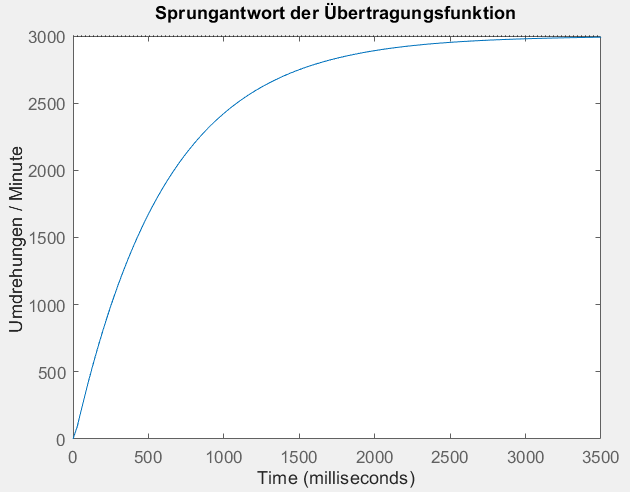
\includegraphics[scale=1.0]{Bilder/Sprungantwort.PNG}
      \captionof{figure}{Sprungantwort 1V}
      \label{fig:Sprungantwort} 
   \end{minipage}
\end{center}






%%
%% Aufgabe 3 - Ermitteln Sie die Anstiegszeit 10% -> 90% des Endwerts
%%

\paragraph{Aufgabe 3 - Anstiegszeit}~\\

Ermitteln Sie die Anstiegszeit 10 \% $\rightarrow$ 90 \% des Endwerts.

Aus der Sprungantwort wird der Endwert 3000 Umdrehunge pro Minute entnommen.
10 \% (300 Umdrehungen pro Minute) sind nach ca. 100 Millisekunden erreicht.
90 \% (2700 Umdrehungen pro Minute) sind nach ca. 1500 Millisekunden erreicht.

Die Differenz entspricht der Anstiegszeit. Sie beträgt 1400 Millisekunden.



%%
%% Aufgabe 4 - Bode-Diagramm
%%

\paragraph{Aufgabe 3 - Bode-Diagramm}~\\

Zeichnen Sie das Bode-Diagramm der Strecke.

\begin{lstlisting}[style=CStyle]
bode(sys)
grid on
\end{lstlisting}

Matlab wählt die auszuwertenden Frequenzen automatisch aus. Eine manuelle Erweiterung der Grenzen (bode(sys, \{0.0001, 1000\}))
hat ergeben, dass außerhalb der von Matlab automatisch gewählten Grenzen keine signifikaten Änderungen mehr stattgefunden haben
und es wurden daher die von Matlab gewählten Grenzen beibehalten.

\begin{center}
   \begin{minipage}[b]{1.0\textwidth}
      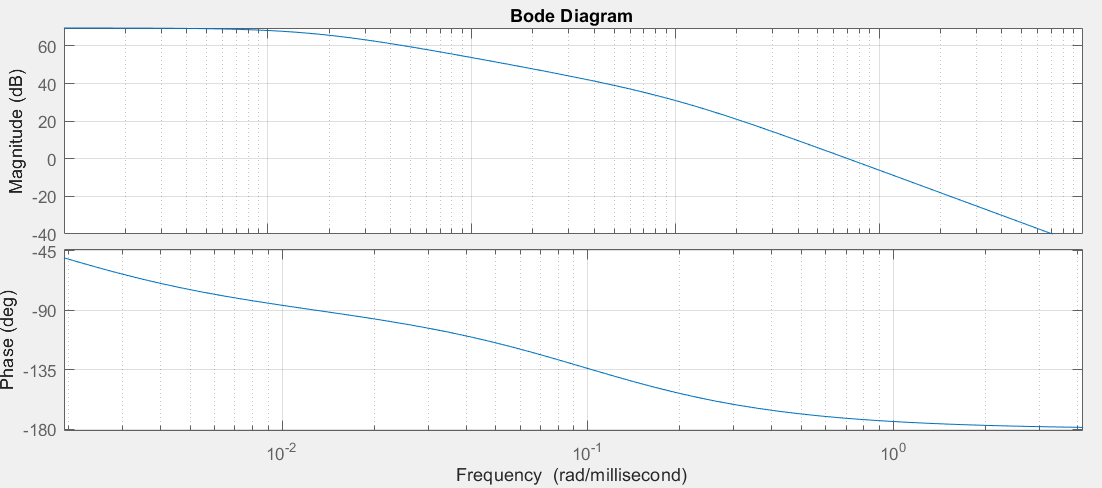
\includegraphics[scale=0.7]{Bilder/Bodeplot.PNG}
      \captionof{figure}{Bode-Diagramm}
      \label{fig:Bodeplot} 
   \end{minipage}
\end{center}

Interessant ist, dass es nicht möglich ist einen Amplitudenrand anzugeben, da die Phase nicht unter 180 Grad fällt.

Der Phasenrand lässt sich bei der Frequenz bestimmen, bei der die Verstärkung der Amplitude 0 ist.
Bei dieser Frequenz beträgt der Phasenrand $-172^{\circ} - -180^{\circ} = 8^{\circ} $

\begin{center}
   \begin{minipage}[b]{1.0\textwidth}
      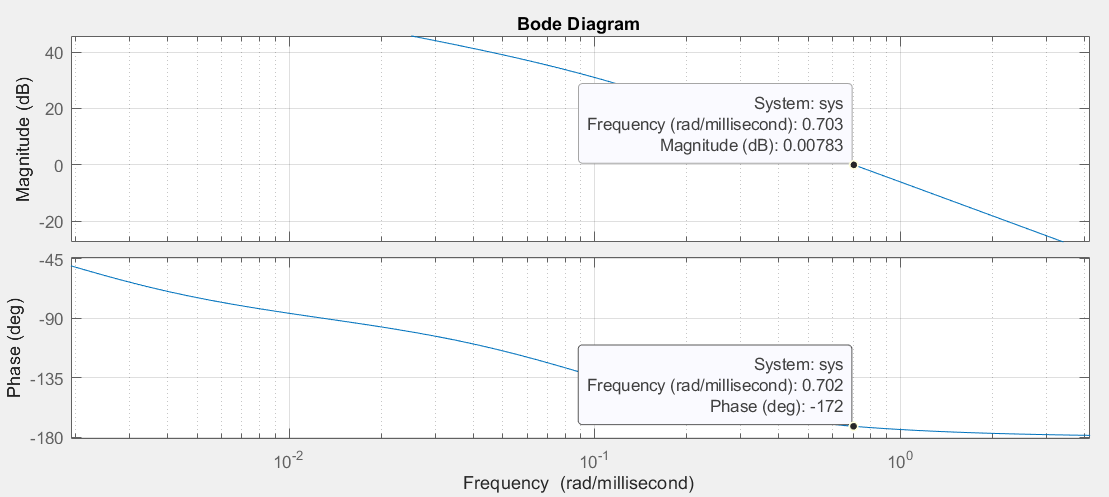
\includegraphics[scale=0.7]{Bilder/Phasenrand.PNG}
      \captionof{figure}{Phasenrand}
      \label{fig:Phasenrand} 
   \end{minipage}
\end{center}

Um das Bode-Diagramm manuell zu zeichnen beginnt man mit dem Amplitudengang.
Es werden einige Frequenzen ausgewählt, da der Zeitaufwand bei der manuellen Berechnung schnell zu hoch wird.
Gewählt werden die Frequenzen $10^{-3}$, $10^{-2}$, $10^{-1}$, $10^{0}$ und $10^{1}$

Diese Werte werden in die Übertragungsfunktion eingesetzt. Aus den Ergebnissen wird dann der Dezibel-Wert gebildet.

\begin{center}
\begin{tabular}{|c c c c|} 
 \hline
 Frequenz & G(s) & log(G(s)) & dB = 20*log(G(s)) \\ [0.5ex] 
 \hline
 $10^{-3}$ & 1856,44 & 3,269 & 65,37 \\
 \hline
 $10^{-2}$ & 389,61 & 2,59 & 51,81 \\
 \hline
 $10^{-1}$ & 24,59 & 1,39 & 27,82 \\
 \hline
 $10^{0}$ & 0,45 & -0.34 & -6.86 \\
 \hline
 $10^{1}$ & $4.94*10^-3$ & -2.31 & -46,11 \\
 \hline
\end{tabular}
\end{center}

TODO: Phasengang




%%
%% Aufgabe 5 - Phasenrand von 70 Grad
%%

\paragraph{Aufgabe 5 - Einstellung Phasenrand}~\\

Ein Phasenrand von 70 Grad soll eingestellt werden.
Der Phasenrand wird im Phasendiagram des Bode-Diagramms an der Stelle abgelesen, an der die Amplitude den Wert 0 annimmt.
Der Phasenrand wird gebildert, indem die Differenz im Phase-Diagramm zwischen dem Kurvenwert und der -180 Grad Linie gebildet wird.

Es ergibt sich aus der Rechnung $70 = x - -180 <=> x = 70 - 180 = -110$ eine Phasenverschiebung von -110 Grad.

Durch Wahl einer Verstärkung K kann die Amplituden-Linie vertikal verschoben werden ohne die Phasen-Linie zu beeinflussen.
Es wird eine Verstärkung K = 0.005 gewählt.

Mit einer Verstärkung von K = 0.005 ergibt sich das Bode-Diagramm \ref{fig:Phasenrand_70Grad}, in dem ein Phasenrand von 70 Grad erreicht ist.

\begin{center}
   \begin{minipage}[b]{0.6\textwidth}
      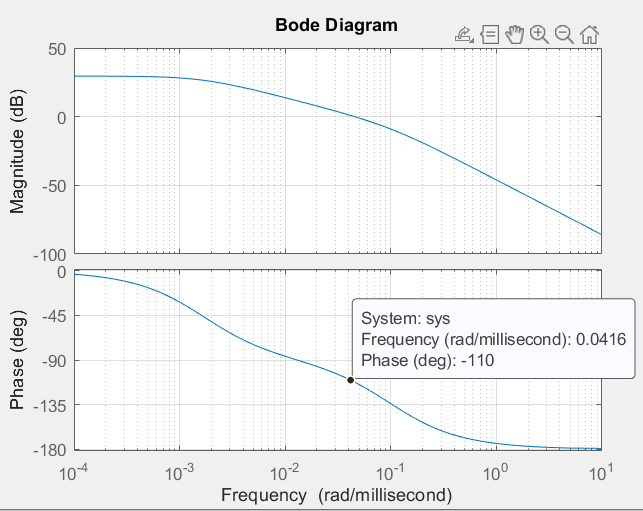
\includegraphics[scale=0.7]{Bilder/Phasenrand_70Grad.PNG}
      \captionof{figure}{Phasenrand}
      \label{fig:Phasenrand_70Grad} 
   \end{minipage}
\end{center}





\newpage
{\let\clearpage\relax \chapter{Abschnitt 4.2 - Simulation des Drehzahlregelkreises}} \label{chpt:SimulationRevolutionControlLoop}

Zunächst wird erklärt, wie die Formel

\begin{equation}
F(j\omega) = \frac{F_r(j\omega)F_s(j\omega)}{1 + F_r(j\omega)F_s(j\omega)}
\end{equation}

zustande kommt. Gegeben ist der Wirkungsplan in \ref{fig:WirkungsplanDrehzahlregelkreis}.

\begin{center}
   \begin{minipage}[b]{0.6\textwidth}
      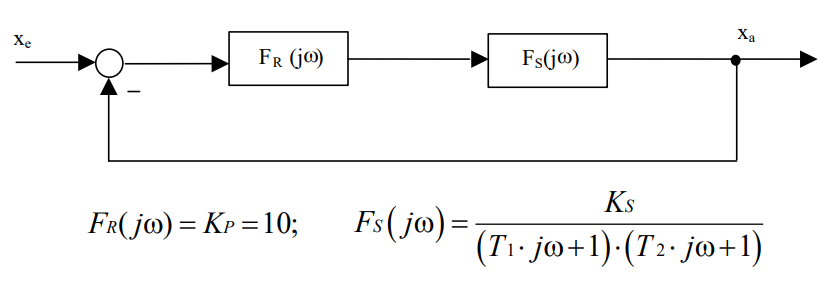
\includegraphics[scale=0.7]{Bilder/WirkungsplanDrehzahlregelkreis.PNG}
      \captionof{figure}{Phasenrand}
      \label{fig:WirkungsplanDrehzahlregelkreis} 
   \end{minipage}
\end{center}

Ein Vergleich mit \cite{Skript_Regelungstechnik} Seite 52 zeigt, dass es sich hier um eine Gegenkopplung handelt, da die Rückführung mit einem negative Vorzeichen an 
den Eingang angelegt wird. 

\begin{center}
   \begin{minipage}[b]{0.9\textwidth}
      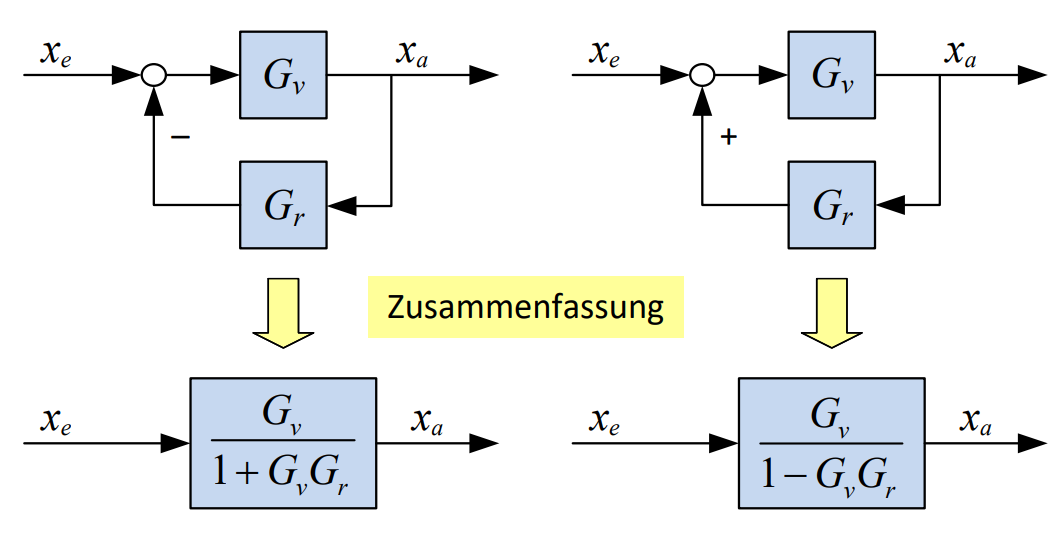
\includegraphics[scale=0.7]{Bilder/GegenUndMitkopplung.PNG}
      \captionof{figure}{Phasenrand}
      \label{fig:GegenUndMitkopplung} 
   \end{minipage}
\end{center}

In \ref{fig:GegenUndMitkopplung}, welche auch \cite{Skript_Regelungstechnik} entnommen ist, wird eine Zusammenfassung der Gegenkopplung in einen einzigen
Block angegeben. Dieser Block wird Formelmäßig durch 

\begin{equation}
F(j\omega) = \frac{G_v(j\omega)}{1 + G_v(j\omega)G_r(j\omega)}
\end{equation}

beschrieben. Um den Wirkungsplan aus der Aufgabe also mit dieser Ersatzformel in Einklang zu bringen, muss $G_r(j\omega)$ als Einheitsfunktion angenommen werden, da
der Wirkungsplan keinen Block im Rückführungszweig enthält.

\begin{equation}
G_r(j\omega) = 1
\end{equation}

Dagegen enthält der Wirkungsplan aus dem Aufgabenblatt (s. Abbildung \ref{fig:WirkungsplanDrehzahlregelkreis}) jedoch zwei Blöcke im Vorwärtszweig, 
nämlich $F_r(j\omega)$ und $F_s(j\omega)$. Diese beiden Blöcke müssen zusammengefasst werden, damit die Formel $F(j\omega) = \frac{G_v(j\omega)}{1 + G_v(j\omega)G_r(j\omega)}$
angewendet werden kann.

Die Regeln der Zusammenfassung sind in \cite{Skript_Regelungstechnik} definiert. Auf Seite 52 wird beschrieben, dass eine Reihenschaltung durch Multiplikation der beiden Blöcke
zu einem Block zusammengefasst werden kann. Es gilt damit:

\begin{equation}
G_v(j\omega) = F_r(j\omega)F_s(j\omega)
\end{equation}

Es folgt nun die Bestimmung des Ersatzblocks aus allen obigen Angaben. Dazu werden $G_v(j\omega)$ und $G_r(j\omega)$ eingesetzt.	

\begin{equation}
F(j\omega) = \frac{G_v(j\omega)}{1 + G_v(j\omega)G_r(j\omega)} = \frac{F_r(j\omega)F_s(j\omega)}{1 + F_r(j\omega)F_s(j\omega) * 1} = \frac{F_r(j\omega)F_s(j\omega)}{1 + F_r(j\omega)F_s(j\omega)}
\end{equation}

Es handelt sich jetzt um die zuvor gesuchte Formel aus der Versuchsanleitung.

Im folgenden wird die Funktion in eine Form gebracht, in der die Zeros und Poles, Gain abgelesen werden können um die Übertragungsfunktion
in Matlab eingeben und ein Bode Diagramm zeichnen zu können.

\begin{equation}
G(j\omega) = \frac{F_r(j\omega)F_s(j\omega)}{1 + F_r(j\omega)F_s(j\omega)} = \frac{\frac{K_{p}K_{s}}{(T_{1}j\omega + 1)(T_{2}j\omega + 1)}}{1 + \frac{K_{p}K_{s}}{(T_{1}j\omega + 1)(T_{2}j\omega + 1)}}
= \frac{\frac{K_{p}K_{s}}{(T_{1}j\omega + 1)(T_{2}j\omega + 1)}}{\frac{(T_{1}j\omega + 1)(T_{2}j\omega + 1) + K_{p}K_{s}}{(T_{1}j\omega + 1)(T_{2}j\omega + 1)}}
\end{equation}

Durch Ausklammer der beiden Verstärkungen $K_{p}$ und $K_{s}$ ergibt sich

\begin{equation}
G(j\omega) = \frac{K_{p}K_{s}}{(T_{1}j\omega + 1)(T_{2}j\omega + 1) + K_{p}K_{s}} = K_{p}K_{s}(\frac{1}{(T_{1}j\omega + 1)(T_{2}j\omega + 1) + 1})
\end{equation}

Wird der Nenner auf Nullstellen untersucht, ergeben sich die Nullstellen $-\frac{1}{10}$ und $-\frac{1}{600}$. Der Nenner wird faktorisiert in

\begin{equation}
G(j\omega) = K_{p}K_{s}( \frac{1}{(j\omega + \frac{1}{10})(j\omega + \frac{1}{600})} )
\end{equation}

Es handelt sich prinzipiell um die gleiche Übertragungsfunktion wie zuvor bis auf den Unterschied, dass der proportionale P-Regler seine Verstärkung $K_{p}$ beiträgt,
die zum $K_{s}$ multipliziert wird.

Die Sprungantwort ist:

\begin{lstlisting}[style=CStyle]
zeros = [];
poles = [-1/10 -1/600];
gain = [10*0.5];
sys = zpk(zeros, poles, gain, 'TimeUnit','milliseconds');

step(sys)
title('Sprungantwort der Uebertragungsfunktion')
xlabel('Time') 
ylabel('Umdrehungen / Minute') 
\end{lstlisting}


\begin{center}
   \begin{minipage}[b]{0.9\textwidth}
      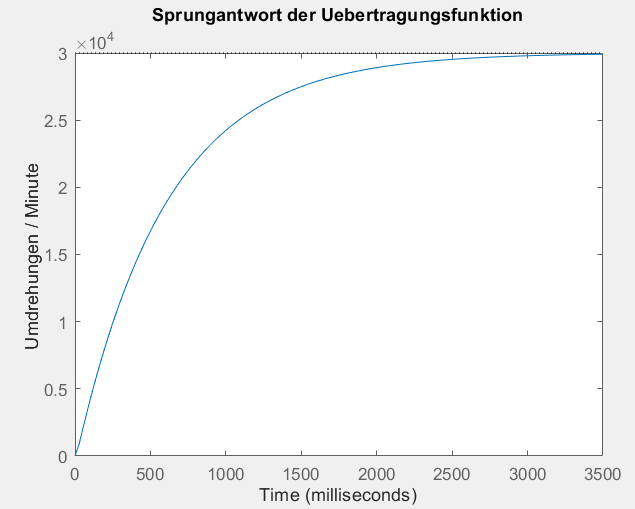
\includegraphics[scale=0.7]{Bilder/Sprungantwort_Gegenkopplung.PNG}
      \captionof{figure}{Phasenrand}
      \label{fig:Sprungantwort_Gegenkopplung} 
   \end{minipage}
\end{center}


\newpage
{\let\clearpage\relax \chapter{Zusammenfassung und Ausblick}} \label{chpt:Conclusion}

Brauchen wir dieses Kapitel?








\bibliographystyle{natdin}
%\bibliographystyle{abbrvnat}
   \bibliography{Literatur/Literatur}        % Bibliographie erzeugen
%   \addtotoc{Quellenverzeichnis}


\end{document}